
\medskip

\section{Illustrative strengths of OOHaskell}
\label{S:strengths}

We would like to highlight some pieces of expressiveness and issues of
convenience implied by our use of Haskell as the base language for OO
programming. Most notably, labels, classes, and methods are all
first-class citizens in OOHaskell, which can be passed as arguments
and returned as results. The combined list that follows is not covered
by any mainstream OO language. This strongly suggests that (OO)Haskell
lends itself as prime environment for typed object-oriented language
design.



%%%%%%%%%%%%%%%%%%%%%%%%%%%%%%%%%%%%%%%%%%%%%%%%%%%%%%%%%%%%%%%%%%%%%%%%%%%%%
%%%%%%%%%%%%%%%%%%%%%%%%%%%%%%%%%%%%%%%%%%%%%%%%%%%%%%%%%%%%%%%%%%%%%%%%%%%%%
%%%%%%%%%%%%%%%%%%%%%%%%%%%%%%%%%%%%%%%%%%%%%%%%%%%%%%%%%%%%%%%%%%%%%%%%%%%%%



\medskip

\subsection{Functions polymorphic in classes}

Consider the following example:

\begin{code}
 myFirstClassOOP point_class =
   do
      p <- mfix (point_class 7)
      p # moveX $ 35
      p # print
 > myFirstClassOOP printable_point
 42
\end{code}
%%% $

\noindent
That is, we have parameterised the function @myFirstClassOOP@ with
respect to a class. We pass @myFirstClassOOP@ a constructor function
(a `class'), which, when instantiated, creates an object with the
slots |move| and |print|. We can pass @myFirstClassOOP@ any
constructor of the class printable point --- or of any other class
provided that the required slots are present. The latter constraint is
statically verified. For instance, our earlier colored point is still
a printable point:

\begin{code}
 ghci> myFirstClassOOP $ flip colored_point "red"
 so far - 42
 color  - "red"
\end{code}
%%% $


%%%%%%%%%%%%%%%%%%%%%%%%%%%%%%%%%%%%%%%%%%%%%%%%%%%%%%%%%%%%%%%%%%%%%%%%%%%%%
%%%%%%%%%%%%%%%%%%%%%%%%%%%%%%%%%%%%%%%%%%%%%%%%%%%%%%%%%%%%%%%%%%%%%%%%%%%%%
%%%%%%%%%%%%%%%%%%%%%%%%%%%%%%%%%%%%%%%%%%%%%%%%%%%%%%%%%%%%%%%%%%%%%%%%%%%%%



\medskip

\subsection{Reusable methods without hosts}

Methods too are first-class citizens in OOHaskell. With a bit of
parameterisation and higher-order functional programming, we can
programme methods outside of any hosting class. Such methods can be
reused across classes without any inheritance relationship.  For
instance, let's identify a method @print_getX@ that can be shared by
all objects that have at least the method @getX@ of type
@Show@~@a@~@=>@~@IO@~@a@~---~regardless of any inheritance
relationships:

\begin{code}
 print_getX self = ((self # getX ) >>= Prelude.print)
\end{code}

\noindent
We can update the code for @printable_point@ as follows:

\begin{code}
 -- before
 ... .*. print    .=. ((s # getX ) >>= Prelude.print)
 -- after
 ... .*. print    .=. print_getX s
\end{code}



%%%%%%%%%%%%%%%%%%%%%%%%%%%%%%%%%%%%%%%%%%%%%%%%%%%%%%%%%%%%%%%%%%%%%%%%%%%%%
%%%%%%%%%%%%%%%%%%%%%%%%%%%%%%%%%%%%%%%%%%%%%%%%%%%%%%%%%%%%%%%%%%%%%%%%%%%%%
%%%%%%%%%%%%%%%%%%%%%%%%%%%%%%%%%%%%%%%%%%%%%%%%%%%%%%%%%%%%%%%%%%%%%%%%%%%%%



\medskip

\subsection{Arbitrarily nested object generators}

Quoting from~\cite[\S\,3.1]{OCaml}:

\begin{quote}\itshape\small
``The evaluation of the body of a class only takes place at object
creation time.  Therefore, in the following example, the instance
variable @varX@ is initialised to different values for two different
objects.''
\end{quote}

\begin{code}
 let x0 = ref 0;;
 val x0 : int ref = {contents = 0}
\end{code}

\begin{code}
 class incrementing_point :
   object
     val mutable varX = incr x0; !x0
     method getX      = varX
     method moveX d   = varX <- varX + d
   end;;
\end{code}

\begin{code}
 new incrementing_point#getX;;
 - : int = 1
 new incrementing_point#getX;;
 - : int = 2
\end{code}

\noindent
Before we transcribe the use of this OCaml idiom to Haskell, we
observe that we can view the body of a class as the body of a
constructor method. Then, any mutable variable that is used along
subsequent invocations of the constructor functionality can be viewed
as belonging to a \emph{class object}.

So we arrive at a nested object generator:

\begin{code}
 incrementing_point = 
   do 
      x0 <- newIORef 0
      returnIO (
        do modifyIORef x0 (+1)
           x <- readIORef x0 >>= newIORef
           returnIO
             $  varX  .=. x
            .*. getX  .=. readIORef x
            .*. moveX .=. (\d -> modifyIORef x ((+) d))
            .*. emptyRecord)
\end{code}
%%% $
\noindent
In general, such nesting could be any number of levels deep since we
just use normal Haskell scopes. In the example, at the outer level, we
do the computation for the point template; at the inner level, we
perform the computation that constructs points themselves. This value
deserves a more OOP-biased name:

\begin{code}
 makeIncrementingPointClass = incrementing_point
\end{code}



%%%%%%%%%%%%%%%%%%%%%%%%%%%%%%%%%%%%%%%%%%%%%%%%%%%%%%%%%%%%%%%%%%%%%%%%%%%%%
%%%%%%%%%%%%%%%%%%%%%%%%%%%%%%%%%%%%%%%%%%%%%%%%%%%%%%%%%%%%%%%%%%%%%%%%%%%%%
%%%%%%%%%%%%%%%%%%%%%%%%%%%%%%%%%%%%%%%%%%%%%%%%%%%%%%%%%%%%%%%%%%%%%%%%%%%%%



\medskip

\subsection{Class closures}

We use the class object from the previous example:

\begin{code}
 myNestedOOP =
   do
      localClass <- makeIncrementingPointClass
      localClass >>= ( # getX ) >>= Prelude.print
      localClass >>= ( # getX ) >>= Prelude.print
 ghci> myNestedOOP
 1
 2
\end{code}
%%% $
\noindent
We effectively created a class in a scope, and then exported it,
closing over a locally-scoped variable. We cannot do such a class
closure in Java! Java supports anonymous objects, but not anonymous
first-class classes. (Nested classes in Java must be linked to an
object of the enclosing class.) C++ is nowhere close to such an
ability.



%%%%%%%%%%%%%%%%%%%%%%%%%%%%%%%%%%%%%%%%%%%%%%%%%%%%%%%%%%%%%%%%%%%%%%%%%%%%%
%%%%%%%%%%%%%%%%%%%%%%%%%%%%%%%%%%%%%%%%%%%%%%%%%%%%%%%%%%%%%%%%%%%%%%%%%%%%%
%%%%%%%%%%%%%%%%%%%%%%%%%%%%%%%%%%%%%%%%%%%%%%%%%%%%%%%%%%%%%%%%%%%%%%%%%%%%%



\medskip

\subsection{Implicit polymorphism}

The class of printable points, given earlier, is polymorphic with
regard to the point's coordinate~---~without our contribution. This is
a fine difference between the OCaml model and our Haskell
transcription. In OCaml's definition of @printable_point@, the
parameter @x_init@ was of the type @int@~---~because the operation
@(+)@ in OCaml can deal with integers only. Our points are
polymorphic~---~a point's coordinate can be any @Num@-ber, for
example, an @Int@ or a @Double@. Here is an example to illustrate
that:

\begin{code}
 myPolyOOP =
   do
      p  <- mfix (printable_point (1::Int))
      p' <- mfix (printable_point (1::Double))
      p  # moveX $ 2
      p' # moveX $ 2.5
      p  # print
      p' # print
\end{code}

\noindent
Our points are actually \emph{bounded} polymorphic. The point
coordinate may be of any type that implements addition. Until very
recently, one could not express this in Java and in C\#. Expressing
bounded polymorphism in C++ is possible with significant
contortions. In (OO)Haskell, we did not have to do anything at
all. Bounded polymorphism (aka, generics) are available in Ada95,
Eiffel and a few other languages. However, in those languages, the
polymorphic type and the type bounds must be declared
\emph{explicitly}. In (OO)Haskell, the type system \emph{infers} the
(bounded) polymorphism on its own.

Of course, implicit polymorphism does not injur static typing. (This
is unlike the poor men's implementation of polymorphic collections,
e.g., in Java @<@ 1.5, which up-casts all the items to the most
general type, @Object@, when inserting elements into the collection,
and which attempts runtime-checked downcasts when accessing elements.) 
Indeed, if we confuse @Int@s and @Double@s in the above code, say we
attempt ``@p@~@#@~@moveX@~@$@~@2.5@'', then we get a type error saying
that @Int@ is not the same as @Double@.

%%% $

 
%%%%%%%%%%%%%%%%%%%%%%%%%%%%%%%%%%%%%%%%%%%%%%%%%%%%%%%%%%%%%%%%%%%%%%%%%%%%%
%%%%%%%%%%%%%%%%%%%%%%%%%%%%%%%%%%%%%%%%%%%%%%%%%%%%%%%%%%%%%%%%%%%%%%%%%%%%%
%%%%%%%%%%%%%%%%%%%%%%%%%%%%%%%%%%%%%%%%%%%%%%%%%%%%%%%%%%%%%%%%%%%%%%%%%%%%%



\begin{figure}[t]
\begin{center}
\resizebox{.45\textwidth}{!}{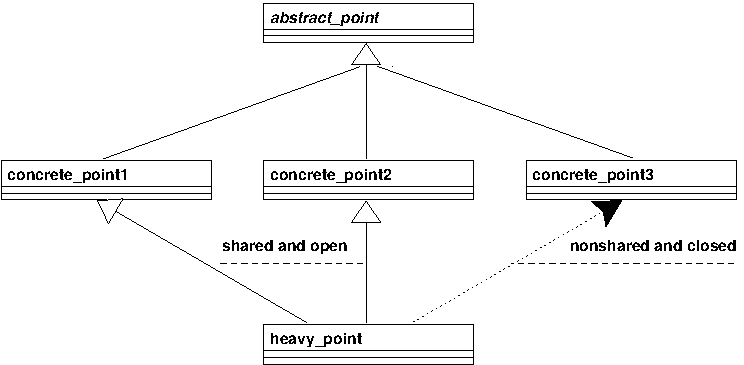
\includegraphics{heavy.pdf}}
\end{center}
\caption{A complex inheritance scenario}
\label{F:heavy}
\end{figure}



%%%%%%%%%%%%%%%%%%%%%%%%%%%%%%%%%%%%%%%%%%%%%%%%%%%%%%%%%%%%%%%%%%%%%%%%%%%%%
%%%%%%%%%%%%%%%%%%%%%%%%%%%%%%%%%%%%%%%%%%%%%%%%%%%%%%%%%%%%%%%%%%%%%%%%%%%%%
%%%%%%%%%%%%%%%%%%%%%%%%%%%%%%%%%%%%%%%%%%%%%%%%%%%%%%%%%%%%%%%%%%%%%%%%%%%%%



\subsection{Programmer-defined inheritance}

In several OO languages, multiple inheritance is allowed. For
instance, in OCaml, the rules are as follows. Only the last definition
of a method is kept: the redefinition in a subclass of a method that
was visible in the parent class overrides the definition in the parent
class. Previous definitions of a method can be reused by binding the
related ancestor using a special \ldots @as@ \ldots notation.  The
bound name is said to be a pseudo value identifier that can only be
used to invoke an ancestor method. Other rules and notations exist for
Eiffel, C++, and so on.

In OOHaskell, the programmer can set up inheritance in flexible ways
taking advantage of the (typed) record calculus. We are going to work
through a scenario, where a class @heavy_point@ is constructed by
inheritance from three different concrete subclasses of
@abstract_point@. The first two concrete points will be shared in the
resulting heavy point, because we leave open the recursive knot. The
third concrete point does not participate in the open recursion; so it
is not shared. See Fig.~\ref{F:heavy} for an overview.

The object template for heavy points starts as follows:

\begin{code}
 heavy_point x_init color self =
  do
     super1 <- concrete_point1 x_init self
     super2 <- concrete_point2 x_init self
     super3 <- mfix (concrete_point3 x_init)
     ... -- to be continued
\end{code}

\noindent
That is, we bind all ancestor objects for subsequent reference. We
pass @self@ to the first two points, which participate in open
recursion, but we fix the third point in place. (Hence, we also
exercise object composition.) A heavy point carries @print@ and
@moveX@ methods that delegate corresponding messages to all three
points:

\begin{code}
     ... -- continued from above
     let myprint = do
                      putStr "super1: "; (super1 # print)
                      putStr "super2: "; (super2 # print)
                      putStr "super3: "; (super3 # print)
     let mymove  = ( \d -> do
                              super1 # moveX $ d
                              super2 # moveX $ d
                              super3 # moveX $ d )
     return 
       $    print  .=. myprint
      .*.   moveX  .=. mymove
      .*.   emptyRecord
     ... -- to be continued
\end{code}

\noindent
The three points, with all their many fields and methods, contribute
to the heavy point by means of left-biased union on records, which is
denoted by ``@.<++.@'' below:

\begin{code}
     ... -- continued from above
      .<++. super1
      .<++. super2
      .<++. super3
\end{code}

Here is a demo:

\begin{code}
 myDiamondOOP =
  do 
     p <- mfix (heavy_point 42 "blue")
     p # print -- All points still agree!
     p # moveX $ 2
     p # print -- The third point lacks behind!
 ghci> myDiamondOOP
 super1: 42
 super2: 42
 super3: 42
 super1: 46
 super2: 46
 super3: 44
\end{code}



%%%%%%%%%%%%%%%%%%%%%%%%%%%%%%%%%%%%%%%%%%%%%%%%%%%%%%%%%%%%%%%%%%%%%%%%%%%%%
%%%%%%%%%%%%%%%%%%%%%%%%%%%%%%%%%%%%%%%%%%%%%%%%%%%%%%%%%%%%%%%%%%%%%%%%%%%%%
%%%%%%%%%%%%%%%%%%%%%%%%%%%%%%%%%%%%%%%%%%%%%%%%%%%%%%%%%%%%%%%%%%%%%%%%%%%%%
 
\medskip

\subsection{Width and depth subtyping}
\label{A:deep}

Suppose you have a class @cube@ and a subclass @cuboid@, which
overrides one of @cube@'s methods by a version with a co-variant
return type (as in Java 5, for example). Substitutability of cubes by
cuboids does not require any casting effort or otherwise. However, we
can coerce a cuboid to become \emph{exactly} of type cube through a
narrowing operation that involves depth subtyping:

\begin{code}
 testDeep = do
   (cuboid::cuboid) <- mfix (class_cuboid
                         (10::Int) (20::Int) (30::Int))
   cube <- mfix (class_cube (40::Int))
   let cuboids = [cuboid, deep'narrow cube]
   putStrLn "Volumes of cuboids"
   mapM_ (\cb -> handle_cuboid cb >>= print) cuboids
\end{code}

The operation @deep'narrow@ must essentially descent into records and
postfix all ``method returns'' by a narrow operation on the results.
There is no magic about the definition of deep subtyping. It is
essentially just another record operation that is driven by the
structure of method types; see the source distribution~\cite{OOHaskell}.



%%%%%%%%%%%%%%%%%%%%%%%%%%%%%%%%%%%%%%%%%%%%%%%%%%%%%%%%%%%%%%%%%%%%%%%%%%%%%
%%%%%%%%%%%%%%%%%%%%%%%%%%%%%%%%%%%%%%%%%%%%%%%%%%%%%%%%%%%%%%%%%%%%%%%%%%%%%
%%%%%%%%%%%%%%%%%%%%%%%%%%%%%%%%%%%%%%%%%%%%%%%%%%%%%%%%%%%%%%%%%%%%%%%%%%%%%


\begin{comment}
\subsection{No equi-recursive types}

Actually, the value recursion IS danagerous, see Remy's Section 3.7. Our
saving grace is that in a call-by-name language fixed-point is always
safe (i.e., it loops). This may be considered just as bad as a
run-time error, but it doesn't force an undefined behavior and
security compromises.

\begin{code}
printable_point1 x_init s =
   do
      x <- newIORef x_init
      s # print
      returnIO
        $  varX  .=. x
       .*. getX  .=. readIORef x
       .*. moveX .=. (\d -> modifyIORef x ((+) d))
       .*. print .=. ((s # getX ) >>= Prelude.print)
       .*. emptyRecord

-- Note that 'mfix' plays the role of 'new' in the OCaml code...
mySelfishOOP1 =
   do
      p <- mfix (printable_point1 7)
      p # moveX $ 2
      p # print
\end{code}
%%% $

When we try mySelfishOOP1, we get |Exception: <<Loop>>|.



It is absolutely not obvious that an object system based on record
calculus can avoid equi-recursive types (whose use is known to
challenge type inference and to complicate a type system
considerably). For instance, Remy's ML-ART calls for recursive types:
``Since objects must be able to send messages to themselves, either
the objects or the functions that send messages to objects have
recursive types''~\cite{ML-ART}.


\ralf{To be honest, I do *not* understand why Remy is right.}

\ralf{Sorry, I also have to give up on the following bits.
I just don't get the fully story.
Let's sort it out on the phone.}

Hence, does OOHaskell circumvent equi-recursive types? We saw that our
class constructor takes @self@ as an argument, and returns the record,
essentially @self'@, as the result. Our encoding (for non-abstract
classes) requires that @self@ and @self'@ have the same slots~---~but
they do not have to be of the same type. This is how we avoid
recursive types. Later on, when we instantiate the class into an
object, we will apply @mfix@ operator -- that is, we will use value
recursion rather than the type recursion. This operation
% mfix, HasField constraint that guarantee mfix is applied to
% something of a record type, the absence of recursive types
% See ML-ART, end of Section 3.1
guarantees safety~\cite{ML-ART} that is, no method accesses fields
that are not filled in yet.

Of course our technique requires that no method type involves the type
of the self argument (\emph{not} counting the implicit self). This is
indeed the case in most OO languages, where we must declare the type
of the argument and the result of a method, and that type must be a
concrete type rather than just `self'.\footnote{\small Functional
objects obviously break this rule. We have found a way to deal with
functional objects while avoiding recursive and existential types, but
this topic is outside of the scope of the present paper.}

\ralf{Perhaps this should go elsewhere}

There is a related issue: the tension between nominal and structural
types. Our record types and therefore our classes provide structural
subtype polymorphism~---~just as in OCaml. Many other OO languages
prefer nominal classes. In OOHaskell, it is trivial to make nominal
distinctions by wrapping structural record types in Haskell
@newtype@s.  One can easily derive a definition for @(#)@ and other
record operations if necessary so that we can operate on nominal types
with the same easy as on structural types. Not surprisingly, we
\emph{must} introduce nominal types in case we deal with recursive
class structures. A type system \emph{with} equi-recursive types would
be slightly more convenient in this respect, while it was injure type
inference at the same time. The source distribution demonstrates the
nominal approach~\cite{OOHaskell}.

\end{comment}
